\documentclass{article}
\usepackage[utf8]{inputenc}
\usepackage{graphicx}
\usepackage{float}
\floatstyle{boxed} 
\restylefloat{figure}
\begin{document}
\title{Exercise 4 of the Computer Vision course at the
  University of Helsinki in May 2018}

\author{\emph{Konsta Kutvonen}}
\maketitle



\newpage
\section{Exercises}
\subsection{Hands-on}
Processing the video with one way nearest neighbour matching took about 0.25 seconds per frame. Changing the algorithm to FLANN reduced the frame processing time down to 0.03 seconds.

\subsection{Homework}
The first parameter provided is the scale factor which specifies how much the image size is reduced every time the image gets scaled. The second parameter is the amount of neighbours an area hast to retain to be considered a candidate at each step.
I looked at cascadeclassifier.cpp, facedetect.cpp and cascadedetect.cpp. 
\subsection{Time}
Handson 3 hours, homework 3 hours.

\section{Code}
\begin{verbatim}
print('Reading images')

post = cv2.imread('poster.jpeg')
fram = cv2.imread('frame.jpeg')
ppl = cv2.imread('people.jpeg')
plt.imshow(ppl)

orb = cv2.ORB_create()

k1, d1 = orb.detectAndCompute(post, None)
k2, d2 = orb.detectAndCompute(fram, None)
print (d1)
k1 = np.array(k1)
k2 = np.array(k2)

plt.imshow(d1)
cv2.imwrite('test.jpeg', d1)

a = post.shape[0]
b = fram.shape[0]
height = max(a, b)
width = post.shape[1]+ fram.shape[1]
img = np.zeros((height, width, 3), np.uint8)

dx = post.shape[1]

for i in range(0, fram.shape[0]):
    for j in range(0, fram.shape[1]):
        img[i][j] = fram[i][j]

for i in range(fram.shape[1], fram.shape[1] + post.shape[0]):
    for j in range(0, fram.shape[0]):
        if j < post.shape[0] and i < img.shape[1]:
            img[j][i] = (post[j][i - fram.shape[1]])
cv2.imwrite('combined.jpeg', img)
plt.imshow(img)

post2 = cv2.imread('poster.jpeg')
fram2 = cv2.imread('frame.jpeg')
gray=cv2.cvtColor(post2, cv2.COLOR_BGR2GRAY)

out1 = cv2.drawKeypoints(post, k1, None, color=(0,255,0))
out2 = cv2.drawKeypoints(fram, k2, None, color=(0,255,0))

cv2.imwrite('test1.jpeg', out1)
cv2.imwrite('test2.jpeg', out2)
plt.imshow(out1)

kn1 = cv2.ml.KNearest_create()
kn2 = cv2.ml.KNearest_create()

kn1.train(np.float32(d1), cv2.ml.ROW_SAMPLE, np.arange(len(d1)))
ret1, res1, nei1, dis1 = kn1.findNearest(np.float32(d2), k=1)

kn2.train(np.float32(d2), cv2.ml.ROW_SAMPLE, np.arange(len(d2)))
ret2, res2, nei2, dis2 = kn2.findNearest(np.float32(d1), k=1)

cp = np.array(img, copy=True)
for i in range (len(res2)):
    (a1, b1) = k1[i].pt
    (a2, b2) = k2[int(res2[i])].pt
    cv2.line(cp, (np.int32(a1 + fram.shape[1]), np.int32(b1)), (np.int32(a2), np.int32(b2)), (0, 255, 0), 1)

plt.imshow(cp)
cv2.imwrite('alllinest.jpeg', cp)

cp = np.array(img, copy=True)
for i in range (len(res1)):
    (a1, b1) = k1[int(res1[i])].pt
    (a2, b2) = k2[i].pt
    for j in range (len(res2)):
        if k1[j].pt ==  k1[int(res1[i])].pt: 
            if k2[int(res2[j])].pt == k2[i].pt:
                cv2.line(cp, (np.int32(a1+ fram.shape[1]), np.int32(b1)), (np.int32(a2), np.int32(b2)), (0, 255, 0), 1)
        
plt.imshow(cp)
cv2.imwrite('linest.jpeg', cp)

FLANN_INDEX_KDTREE = 0
index_params = dict(algorithm = 6,
                   table_number = 6, # 12
                   key_size = 12,     # 20
                   multi_probe_level = 1) #2
search_params = dict(checks=50)   # or pass empty dictionary

flann = cv2.FlannBasedMatcher(index_params, search_params)
matches = flann.knnMatch(d1, d2, k=1)


matchesMask = [[0,0] for i in range(len(matches))]

for i in range(0, (len(matches) - 1)):
    m = matches[i][0]
    n = matches[i + 1][0]
    if m.distance < 0.7*n.distance:
        matchesMask[i]=[1,0]

draw_params = dict(matchColor = (0,255,0),
                   singlePointColor = (255,0,0),
                   matchesMask = matchesMask,
                   flags = 0)

img3 = cv2.drawMatchesKnn(post, k1, fram, k2,matches,None,**draw_params)

cv2.imwrite('test.jpeg', img3)
plt.imshow(img3,),plt.show()
face_cascade = cv2.CascadeClassifier('./haarcascade_frontalface_default.xml')
prof_cascade = cv2.CascadeClassifier('./haarcascade_profileface.xml')
face_cascade2 = cv2.CascadeClassifier('./haarcascade_frontalface_default.xml')
eye_cascade = cv2.CascadeClassifier('./haarcascade_eye.xml')
glass_cascade = cv2.CascadeClassifier('./haarcascade_eye_tree_eyeglasses.xml')
body_cascade = cv2.CascadeClassifier('./haarcascade_upperbody.xml')
smile_cascade =  cv2.CascadeClassifier('./haarcascade_smile.xml')

nh = cv2.imread('nohands.jpg')
dp = cv2.imread('dp.jpg')
hb = cv2.imread('hb.jpg')
gray = cv2.cvtColor(dp, cv2.COLOR_BGR2GRAY)
# gray = cv2.cvtColor(nh, cv2.COLOR_BGR2GRAY)
# gray = cv2.cvtColor(dp, cv2.COLOR_BGR2GRAY)
# gray = cv2.cvtColor(hb, cv2.COLOR_BGR2GRAY)
plt.imshow(gray)
# faces = prof_cascade.detectMultiScale(gray)
faces = face_cascade.detectMultiScale(gray, 1.1, 2)
img = np.array(dp, copy=True)
for (x,y,w,h) in faces:
    cv2.rectangle(img,(x,y),(x+w,y+h),(255,0,0) ,2)
    roi_gray = gray[y:y+h, x:x+w]
    roi_color = img[y:y+h, x:x+w]
#     eyes = eye_cascade.detectMultiScale(roi_gray, 1.1, 2)
    eyes = smile_cascade.detectMultiScale(roi_gray, 1.6, 2)
    for (ex,ey,ew,eh) in eyes:
        cv2.rectangle(roi_color,(ex,ey),(ex+ew,ey+eh),(0,255,0),2)
plt.imshow(img)
cv2.imwrite('dpfaceeye.jpeg', img)


import cv2
import numpy as np
from datetime import datetime
from matplotlib import pyplot as plt
import math

cap = cv2.VideoCapture('video.avi')
orb = cv2.ORB_create()
kn1 = cv2.ml.KNearest_create()
post = cv2.imread('poster.jpeg')
k1, d1 = orb.detectAndCompute(post, None)
kn1.train(np.float32(d1), cv2.ml.ROW_SAMPLE, np.arange(len(d1)))
while(True):
    ret, frame = cap.read()
    cp = np.array(frame, copy=True)
    a = datetime.now()

    kk, dd = orb.detectAndCompute(frame, None)
    if dd is None: break
    ret, res, nei, dis = kn1.findNearest(np.float32(dd), k=1)
    for i in range(0, post.shape[1]):
        for j in range(0, post.shape[0]):
            if j < post.shape[0] and i < post.shape[1]:
                cp[j][i] = (post[j][i])
    for i in range (len(res)):
        (a1, b1) = k1[int(res[i])].pt
        (a2, b2) = kk[i].pt
        cv2.line(cp, (np.int32(a1), np.int32(b1)), (np.int32(a2), np.int32(b2)), (0, 255, 0), 1)



    # index_params = dict(algorithm = 6,
    #                    table_number = 6, # 12
    #                    key_size = 12,     # 20
    #                    multi_probe_level = 1) #2
    # search_params = dict(checks=50)   # or pass empty dictionary
    #
    # flann = cv2.FlannBasedMatcher(index_params, search_params)
    # matches = flann.knnMatch(d1, dd, k=1)
    #
    #
    # matchesMask = [[0,0] for i in range(len(matches))]
    #
    # for i in range(0, (len(matches) - 2)):
    #     m = matches[i]
    #     n = matches[i + 1]
    #     if len(n) > 0 and len(m) > 0:
    #         n = n[0]
    #         m = m[0]
    #         if m.distance < 0.7*n.distance:
    #             matchesMask[i]=[1,0]
    #
    # draw_params = dict(matchColor = (0,255,0),
    #                    singlePointColor = (255,0,0),
    #                    matchesMask = matchesMask,
    #                    flags = 0)
    #
    # img3 = cv2.drawMatchesKnn(post, k1, frame, kk ,matches,None,**draw_params)

    cv2.imshow('title', cp)

    cv2.imwrite('frameslow.jpeg', cp)
    b = datetime.now()
    c = b - a
    print(c.total_seconds())
    cv2.waitKey(0)

cap.release()
cv2.destroyAllWindows()


# import cv2
# import sys
#
# faceCascade = cv2.CascadeClassifier('./haarcascade_frontalface_default.xml')
#
# video_capture = cv2.VideoCapture(0)
#
# while True:
#     # Capture frame-by-frame
#     ret, frame = video_capture.read()
#
#     gray = cv2.cvtColor(frame, cv2.COLOR_BGR2GRAY)
#
#     faces = faceCascade.detectMultiScale(
#         gray,
#         scaleFactor=1.1,
#         minNeighbors=5,
#         minSize=(30, 30)
#     )
#
#     # Draw a rectangle around the faces
#     for (x, y, w, h) in faces:
#         cv2.rectangle(frame, (x, y), (x+w, y+h), (0, 255, 0), 2)
#
#     # Display the resulting frame
#     cv2.imshow('Video', frame)
#
#     if cv2.waitKey(1) & 0xFF == ord('q'):
#         break
#
# # When everything is done, release the capture
# video_capture.release()
# cv2.destroyAllWindows()

\end{verbatim}
\newpage

\begin{figure}
\center
            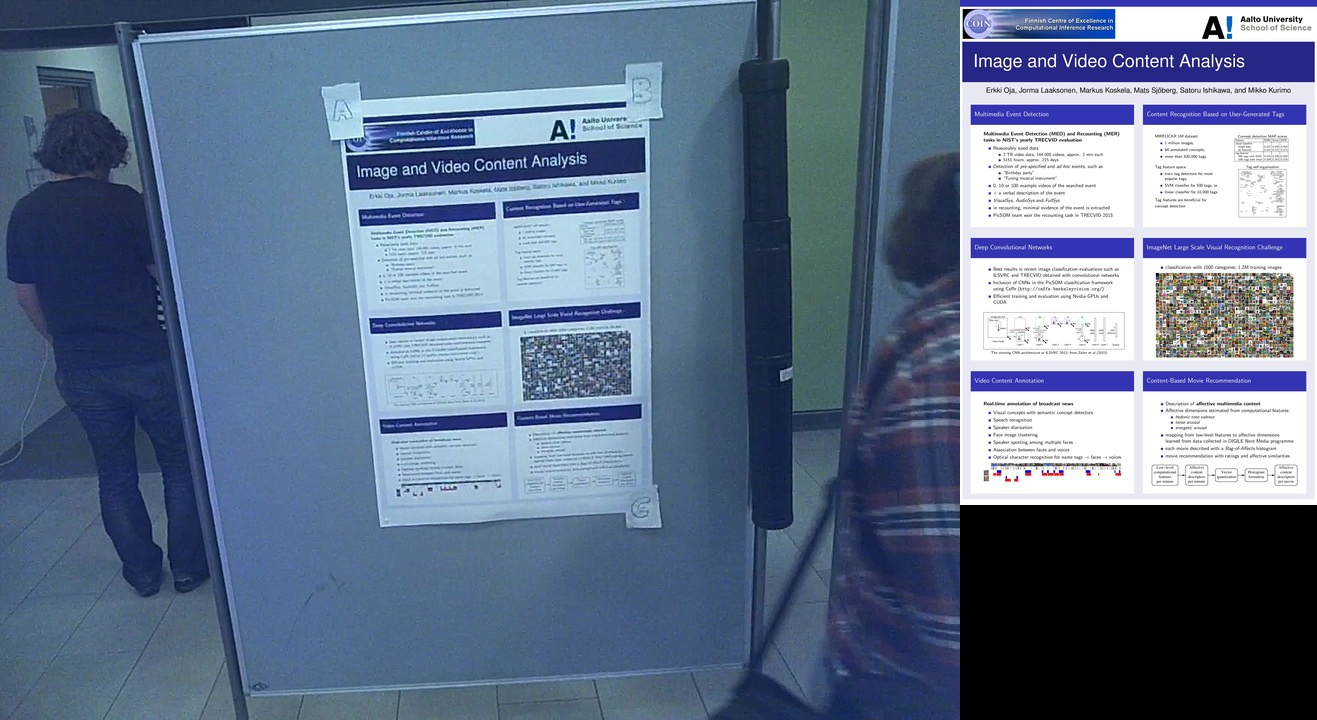
\includegraphics[width=0.6\textwidth]{combined}
\caption{Two images stitched to one}
\end{figure}        
\begin{figure}
\center
            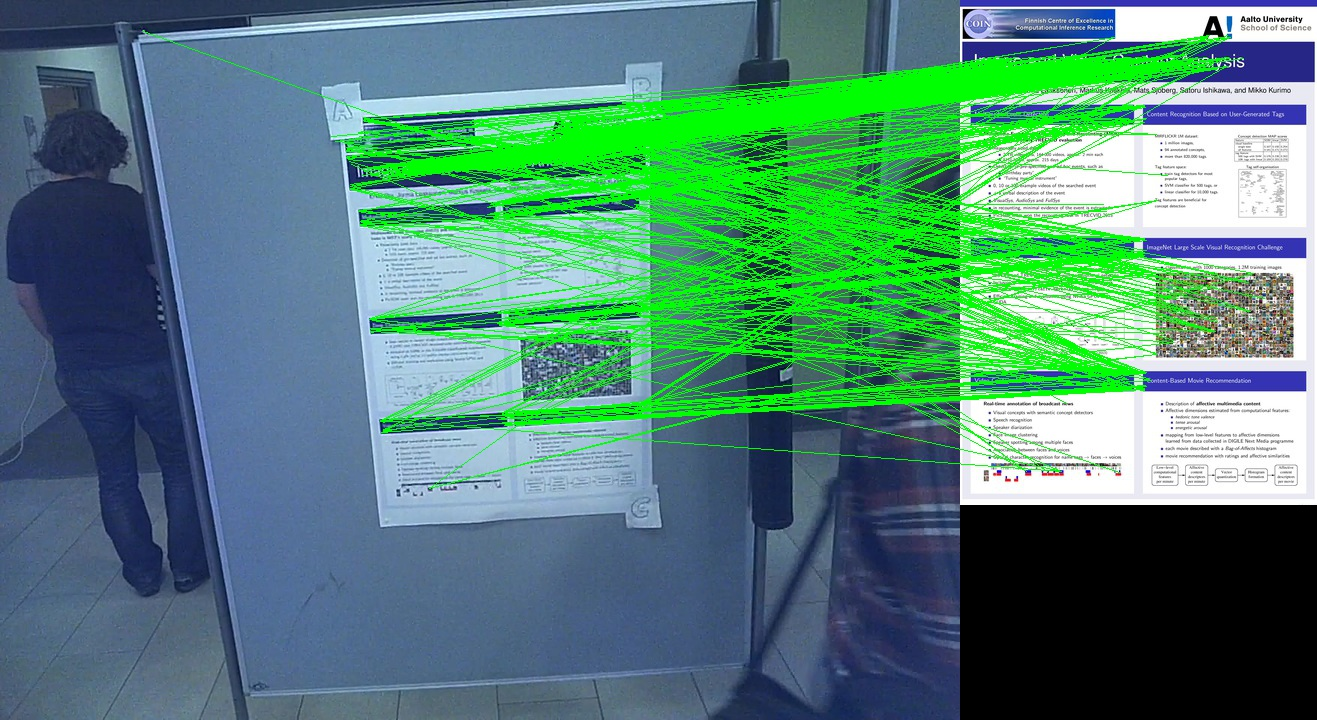
\includegraphics[width=0.6\textwidth]{alllines}
\caption{All lines from the poster to frame}
\end{figure}        
\begin{figure}
\center
            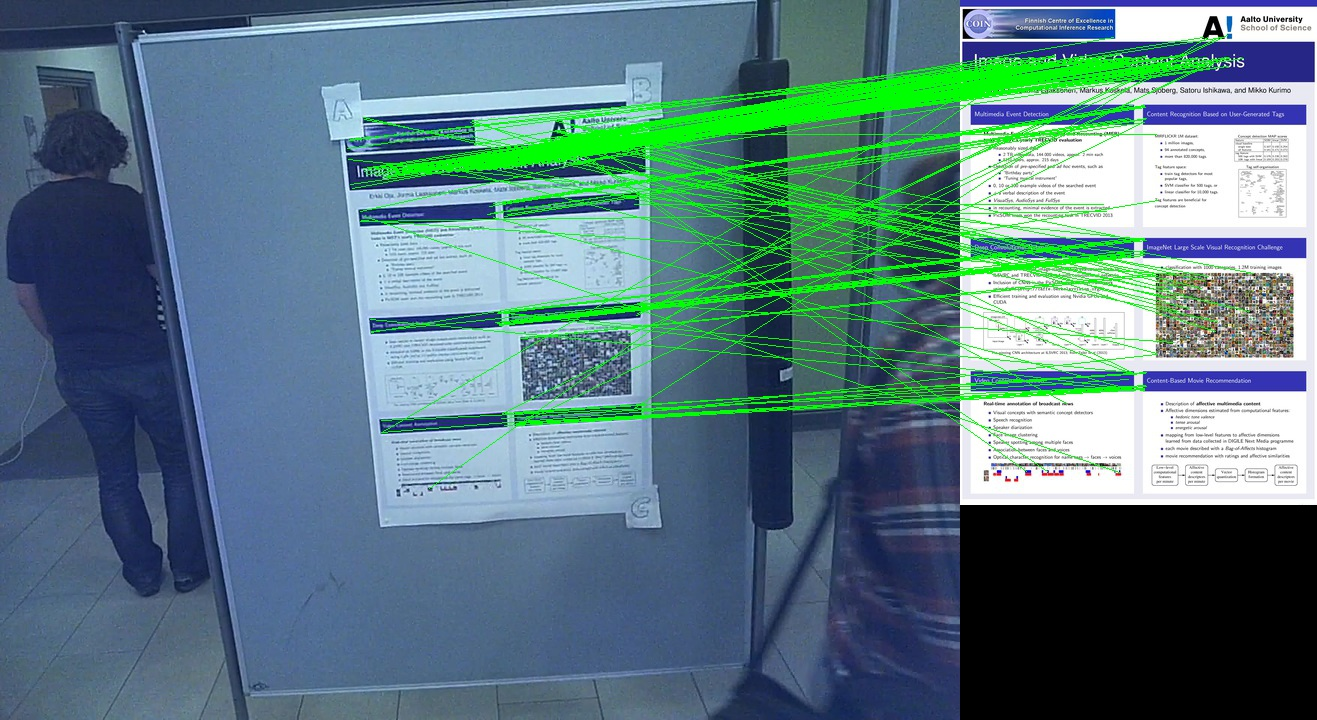
\includegraphics[width=0.6\textwidth]{linest}
\caption{Two way matched}
\end{figure}    

\begin{figure}
\center
            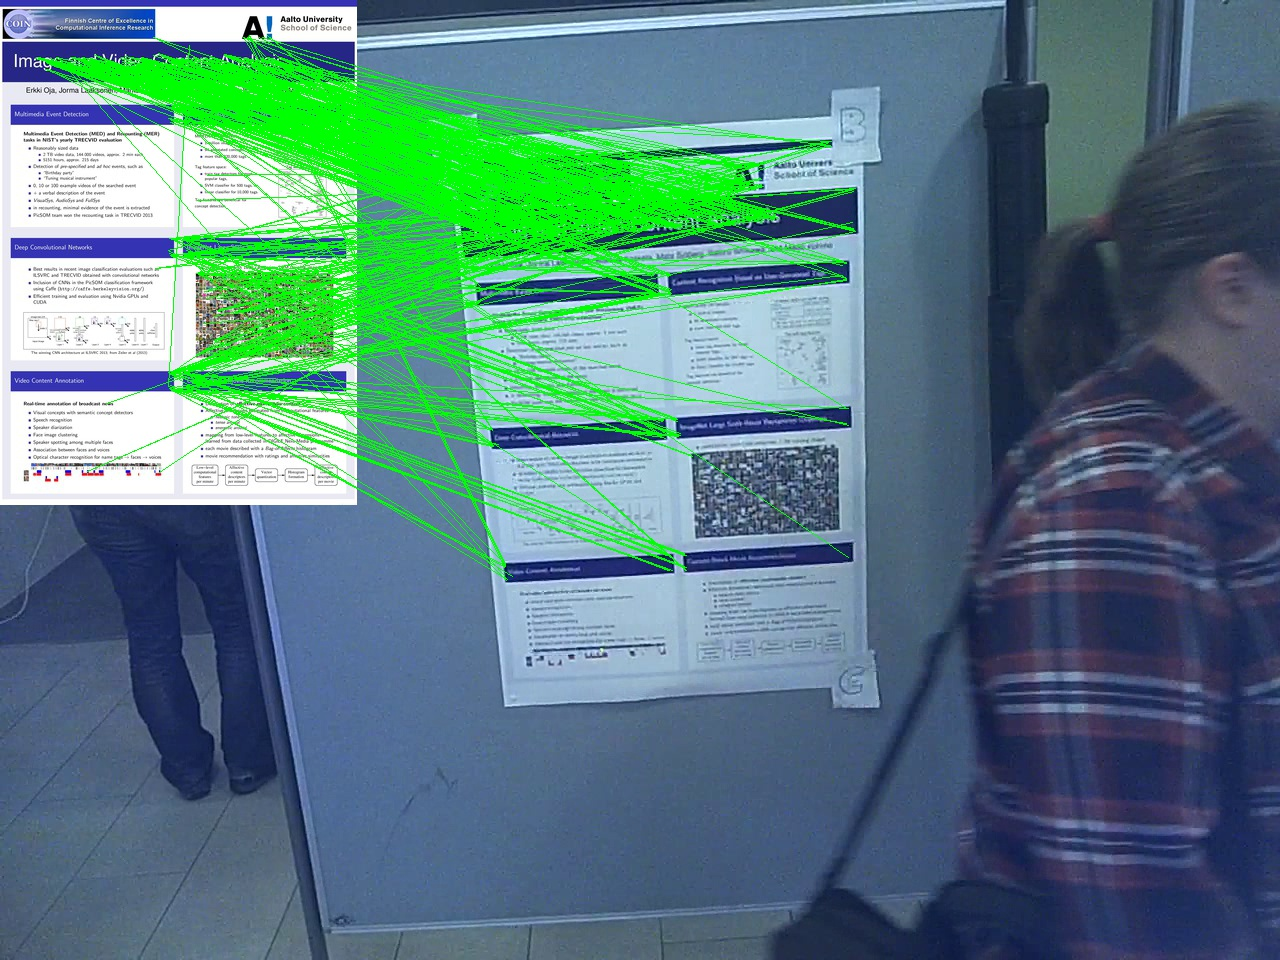
\includegraphics[width=1\textwidth]{frameslow}
\caption{One way nn matching video frame}
\end{figure}        
\begin{figure}
\center
            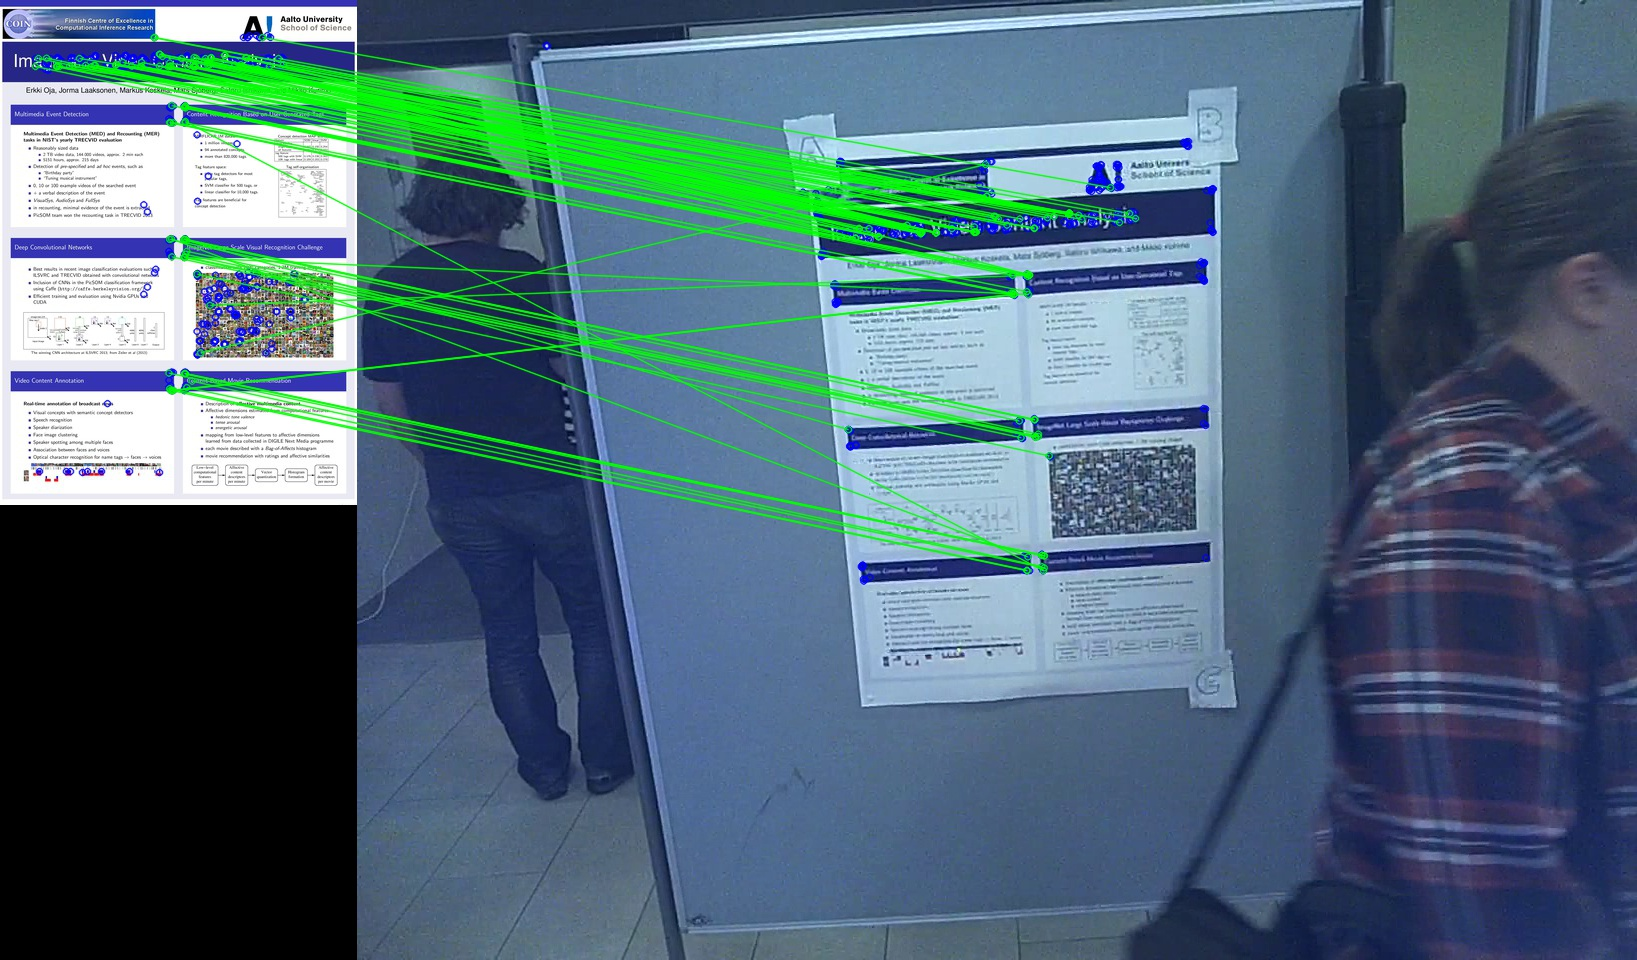
\includegraphics[width=1\textwidth]{flannv}
\caption{Flann video frame}
\end{figure}         
\begin{figure}
\center
            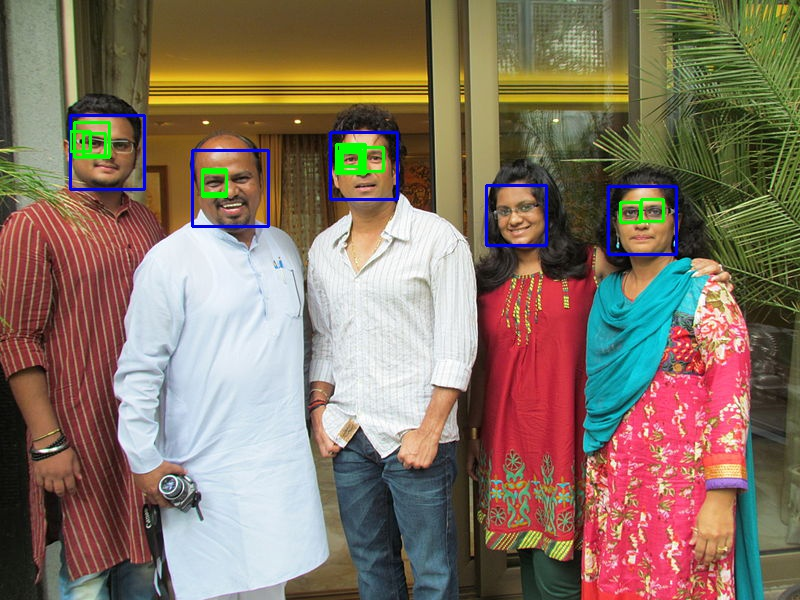
\includegraphics[width=1\textwidth]{pplface}
\caption{Detecting eyes and faces}
\end{figure}      
\begin{figure}
\center
            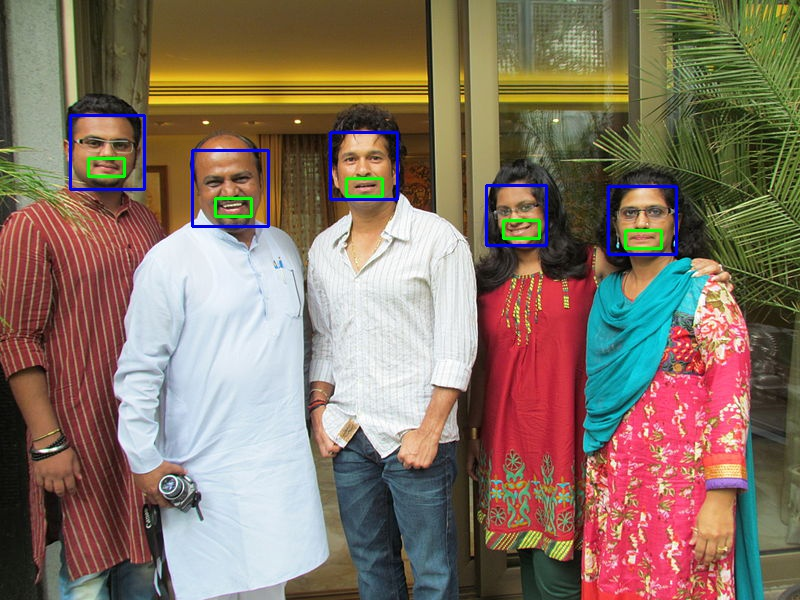
\includegraphics[width=1\textwidth]{pplfacesmile}
\caption{Detecting faces and smiles}
\end{figure}     
\begin{figure}
\center
            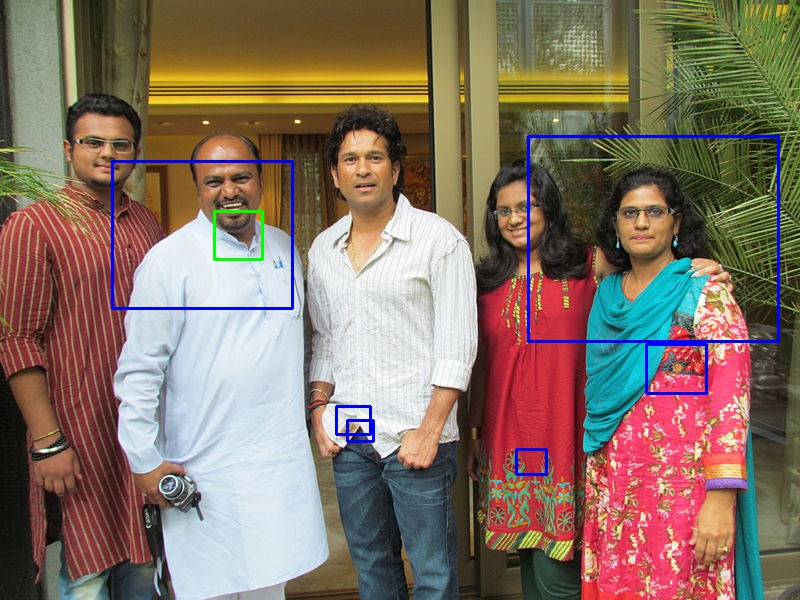
\includegraphics[width=1\textwidth]{pplub}
\caption{Upper body detection}
\end{figure}      
\begin{figure}
\center
            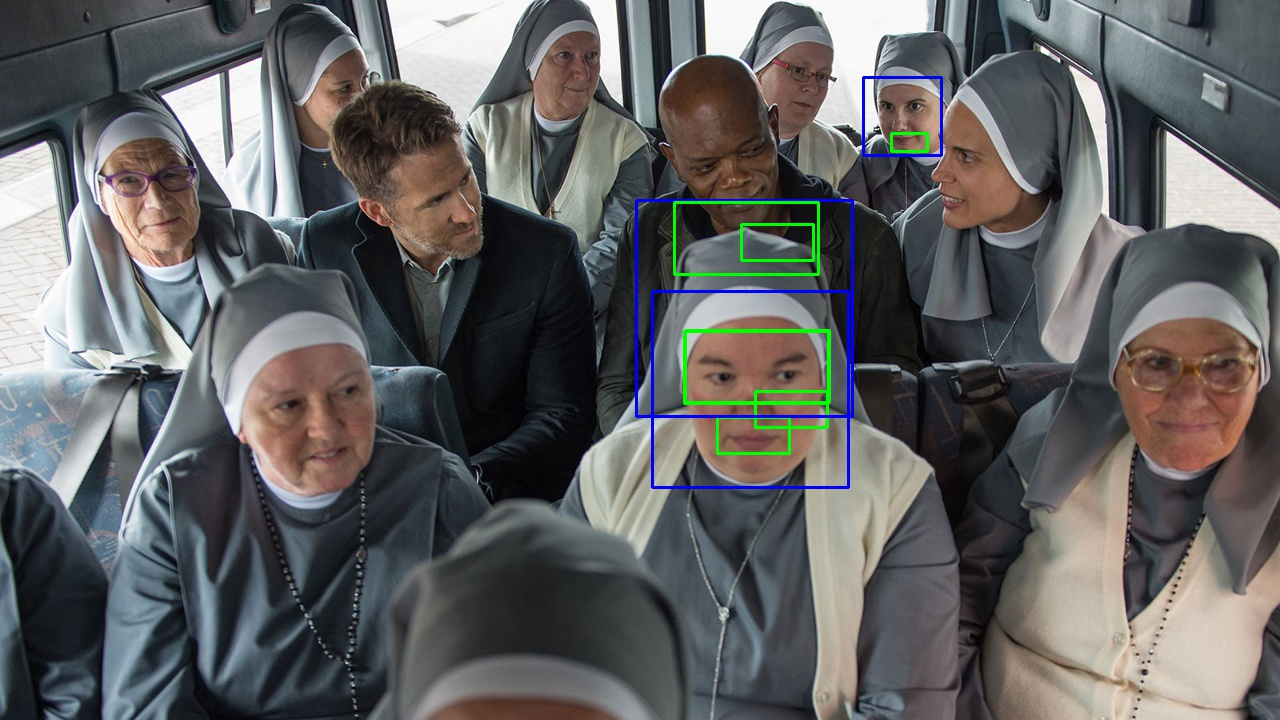
\includegraphics[width=1\textwidth]{hbd}
\caption{Detecting faces and smiles with normal face detector}
\end{figure}       
\begin{figure}
\center
            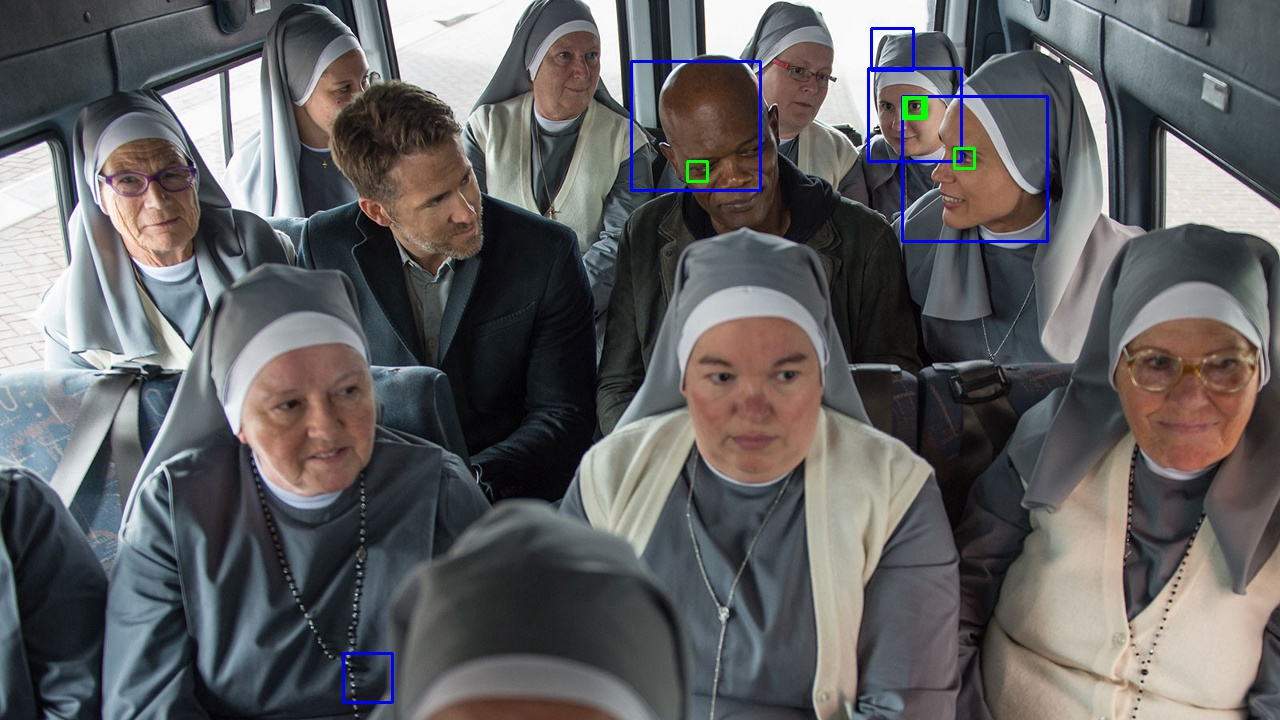
\includegraphics[width=1\textwidth]{hbp}
\caption{Detecting faces and eyes with profile face detector}
\end{figure}       
\begin{figure}
\center
            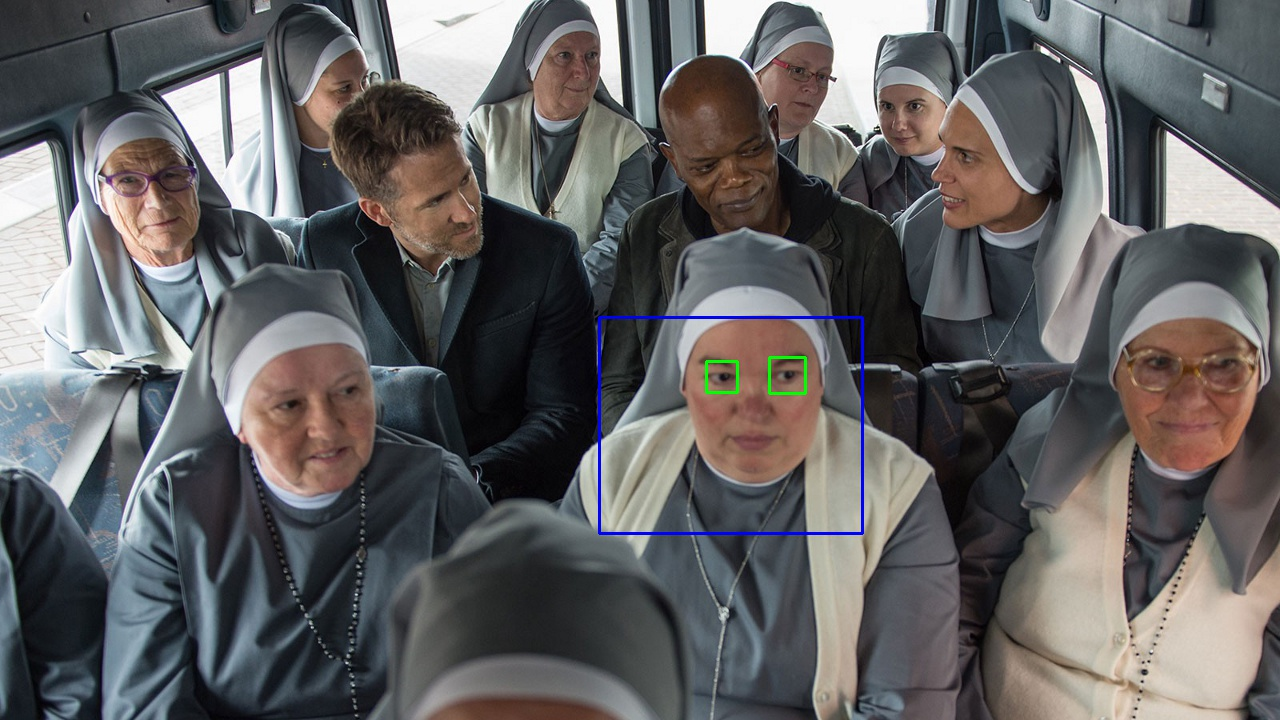
\includegraphics[width=1\textwidth]{hbub}
\caption{Detecting upper bodies and eyes}
\end{figure}  
\begin{figure}
\center
            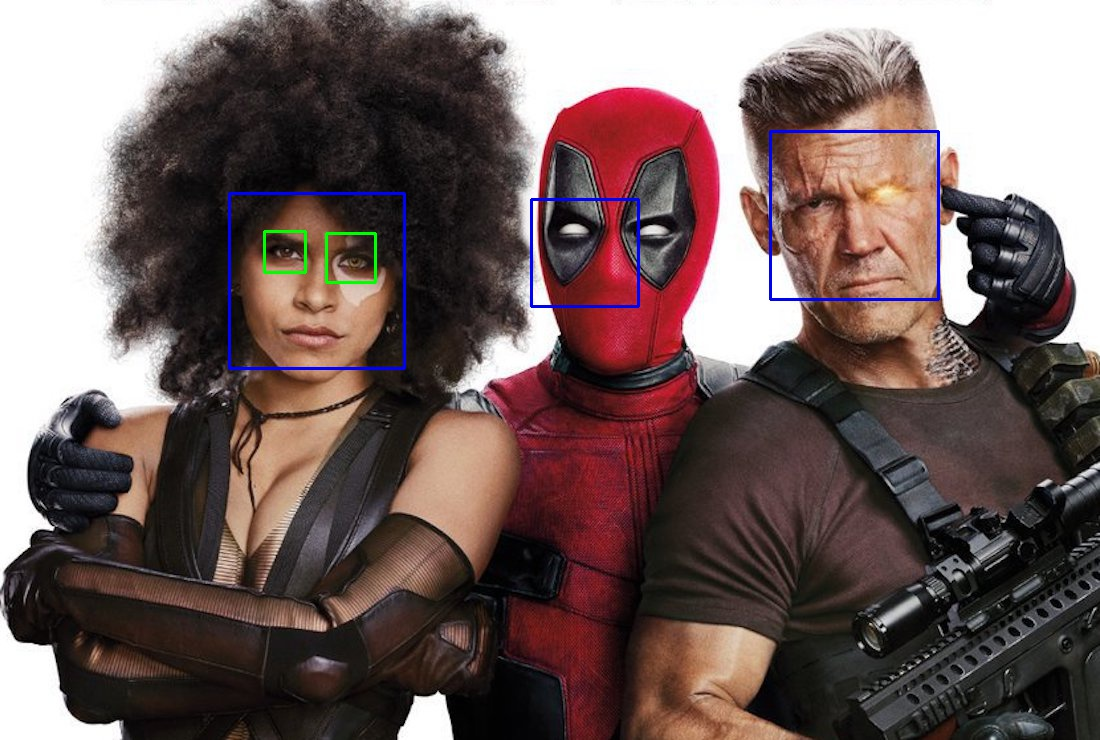
\includegraphics[width=1\textwidth]{dpfacesmile}
\caption{Faces and eyes detection}
\end{figure}       
\end{document}
